\section{Teilversuch 4: Induktion durch ein zeitlich veränderliches Magnetfeld}
	Aus dem Ohmschen Gesetz gilt:
	\begin{align}
		U = I\!R  && \Leftrightarrow && I = \frac{U}{R}
	\end{align}
	Im Experiment haben wir als Widerstand \SI{0.150(2)}{\ohm}, somit skalieren wir die Abszisse mit $1/\SI{0.150}{\ohm}$:
	\begin{align}
		y-\text{Skala} = \frac{\SI{20}{\milli\volt\per\centi\meter}}{\SI{0.150}{\ohm}} = 133\frac{1}{3} \si{\milli\ampere\per\centi\meter} = \frac{\SI{400}{\milli\ampere}}{\SI{3}{\centi\meter}}
	\end{align}
	Aus dem Schreiberdiagramme 
	\begin{equation*}
		\begin{tabu}{l|ll|ll}
			\toprule
			\text{Kurve} & \text{Punkt } 1 & \text{Punkt } 2 & \text{Steigung}/\si{\milli\ampere\per\second} & U_{\text{ind}} \\
			\midrule
			\Circled{1} & (9,30 , 940,0) & (20,60 , -820,0) & -155,8 & 110,0\\
			\Circled{2} & (8,15 , 840,0) & (22,00 , -840,0) & -121,3 & 84,0\\
			\Circled{3} & (7,85 , 720,0) & (22,60 , -740,0) & -98,98 & 70,0\\
			\Circled{4} & (5,35 , 780,0) & (23,70 , -700,0) & -80,65 & 54,0\\
			\Circled{5} & (4,30 , 500,0) & (24,50 , -440,0) & -46,53 & 32,0\\
			\bottomrule
		\end{tabu}
	\end{equation*}
	\includepdf{./scans/tv4.pdf}
	% Zur Induktionsspannung:
	% \begin{equation*}
	% 	\begin{tabu}{l *{5}{l}}
	% 		\toprule
	% 		\text{Kurve} & \Circled{1} & \Circled{2} & \Circled{3} & \Circled{4} & \Circled{5}\\
	% 		\midrule
	% 		U_{\text{ind}}/\si{\milli\volt} &  \\
	% 		\bottomrule
	% 	\end{tabu}
	% \end{equation*}
	Aus dem Induktionsgesetz gilt:
	\begin{align}
		U_{\text{ind}} &= - N_{\text{ind}} \dv{}{t}\left(\vec{B} \cdot \vec{A}\,\right) = -N_{\text{ind}}A \dv{B}{t} = -N_{\text{ind}}A\mu_0\left(\frac{4}{5}\right)^{\nicefrac{3}{2}} \frac{N}{r}\cdot\dv{I}{t} \notag \\
		\Rightarrow U_{\text{ind}} &= \left[-\left(\frac{4}{5}\right)^{\nicefrac{3}{2}} \frac{2\mu_0N_{\text{ind}}N\!A}{R}\right]\cdot\dv{I}{t}
	\end{align}
	Also ist $U_{\text{ind}}$ proportional zu $\displaystyle \dv{I}{t}$, mit $R = $ Durchmesser wie im Teilversuch $3$.

	Die induzierte Spannung $U_{\text{ind}}$ wurde dann gegen die Steigung $\displaystyle \dv{I}{t}$ im \gnuplot{} geplottet und eine Kurveanpassung zur $\displaystyle U_{\text{ind}} = m\dv{I}{t} + c$ durchgeführt. Der Fehler der jeweiligen Punkten sind hier nicht berücksichtigt:
	\begin{figure}[H]
		\centering
		% GNUPLOT: LaTeX picture with Postscript
\begingroup
  \makeatletter
  \providecommand\color[2][]{%
    \GenericError{(gnuplot) \space\space\space\@spaces}{%
      Package color not loaded in conjunction with
      terminal option `colourtext'%
    }{See the gnuplot documentation for explanation.%
    }{Either use 'blacktext' in gnuplot or load the package
      color.sty in LaTeX.}%
    \renewcommand\color[2][]{}%
  }%
  \providecommand\includegraphics[2][]{%
    \GenericError{(gnuplot) \space\space\space\@spaces}{%
      Package graphicx or graphics not loaded%
    }{See the gnuplot documentation for explanation.%
    }{The gnuplot epslatex terminal needs graphicx.sty or graphics.sty.}%
    \renewcommand\includegraphics[2][]{}%
  }%
  \providecommand\rotatebox[2]{#2}%
  \@ifundefined{ifGPcolor}{%
    \newif\ifGPcolor
    \GPcolortrue
  }{}%
  \@ifundefined{ifGPblacktext}{%
    \newif\ifGPblacktext
    \GPblacktexttrue
  }{}%
  % define a \g@addto@macro without @ in the name:
  \let\gplgaddtomacro\g@addto@macro
  % define empty templates for all commands taking text:
  \gdef\gplbacktext{}%
  \gdef\gplfronttext{}%
  \makeatother
  \ifGPblacktext
    % no textcolor at all
    \def\colorrgb#1{}%
    \def\colorgray#1{}%
  \else
    % gray or color?
    \ifGPcolor
      \def\colorrgb#1{\color[rgb]{#1}}%
      \def\colorgray#1{\color[gray]{#1}}%
      \expandafter\def\csname LTw\endcsname{\color{white}}%
      \expandafter\def\csname LTb\endcsname{\color{black}}%
      \expandafter\def\csname LTa\endcsname{\color{black}}%
      \expandafter\def\csname LT0\endcsname{\color[rgb]{1,0,0}}%
      \expandafter\def\csname LT1\endcsname{\color[rgb]{0,1,0}}%
      \expandafter\def\csname LT2\endcsname{\color[rgb]{0,0,1}}%
      \expandafter\def\csname LT3\endcsname{\color[rgb]{1,0,1}}%
      \expandafter\def\csname LT4\endcsname{\color[rgb]{0,1,1}}%
      \expandafter\def\csname LT5\endcsname{\color[rgb]{1,1,0}}%
      \expandafter\def\csname LT6\endcsname{\color[rgb]{0,0,0}}%
      \expandafter\def\csname LT7\endcsname{\color[rgb]{1,0.3,0}}%
      \expandafter\def\csname LT8\endcsname{\color[rgb]{0.5,0.5,0.5}}%
    \else
      % gray
      \def\colorrgb#1{\color{black}}%
      \def\colorgray#1{\color[gray]{#1}}%
      \expandafter\def\csname LTw\endcsname{\color{white}}%
      \expandafter\def\csname LTb\endcsname{\color{black}}%
      \expandafter\def\csname LTa\endcsname{\color{black}}%
      \expandafter\def\csname LT0\endcsname{\color{black}}%
      \expandafter\def\csname LT1\endcsname{\color{black}}%
      \expandafter\def\csname LT2\endcsname{\color{black}}%
      \expandafter\def\csname LT3\endcsname{\color{black}}%
      \expandafter\def\csname LT4\endcsname{\color{black}}%
      \expandafter\def\csname LT5\endcsname{\color{black}}%
      \expandafter\def\csname LT6\endcsname{\color{black}}%
      \expandafter\def\csname LT7\endcsname{\color{black}}%
      \expandafter\def\csname LT8\endcsname{\color{black}}%
    \fi
  \fi
    \setlength{\unitlength}{0.0500bp}%
    \ifx\gptboxheight\undefined%
      \newlength{\gptboxheight}%
      \newlength{\gptboxwidth}%
      \newsavebox{\gptboxtext}%
    \fi%
    \setlength{\fboxrule}{0.5pt}%
    \setlength{\fboxsep}{1pt}%
\begin{picture}(8640.00,5760.00)%
    \gplgaddtomacro\gplbacktext{%
      \csname LTb\endcsname%%
      \put(814,704){\makebox(0,0)[r]{\strut{}$30$}}%
      \put(814,1221){\makebox(0,0)[r]{\strut{}$40$}}%
      \put(814,1738){\makebox(0,0)[r]{\strut{}$50$}}%
      \put(814,2255){\makebox(0,0)[r]{\strut{}$60$}}%
      \put(814,2772){\makebox(0,0)[r]{\strut{}$70$}}%
      \put(814,3289){\makebox(0,0)[r]{\strut{}$80$}}%
      \put(814,3806){\makebox(0,0)[r]{\strut{}$90$}}%
      \put(814,4323){\makebox(0,0)[r]{\strut{}$100$}}%
      \put(814,4840){\makebox(0,0)[r]{\strut{}$110$}}%
      \put(946,484){\makebox(0,0){\strut{}$-160$}}%
      \put(2162,484){\makebox(0,0){\strut{}$-140$}}%
      \put(3378,484){\makebox(0,0){\strut{}$-120$}}%
      \put(4595,484){\makebox(0,0){\strut{}$-100$}}%
      \put(5811,484){\makebox(0,0){\strut{}$-80$}}%
      \put(7027,484){\makebox(0,0){\strut{}$-60$}}%
      \put(8243,484){\makebox(0,0){\strut{}$-40$}}%
    }%
    \gplgaddtomacro\gplfronttext{%
      \csname LTb\endcsname%%
      \put(209,2901){\rotatebox{-270}{\makebox(0,0){\strut{}Induzierte Spannung $U_{\text{ind}}$ $(\si{\milli\volt})$}}}%
      \put(4594,154){\makebox(0,0){\strut{}Gradient des Stromfelds $\displaystyle \dv{I}{t}$ $(\si{\milli\ampere\per\second})$}}%
      \csname LTb\endcsname%%
      \put(7256,4893){\makebox(0,0)[r]{\strut{}$-0,71645 \dv{I}{t} + (-2,11226)$}}%
      \csname LTb\endcsname%%
      \put(7256,4607){\makebox(0,0)[r]{\strut{}Messpunkte}}%
      \csname LTb\endcsname%%
      \put(4594,5429){\makebox(0,0){\strut{}Induzierte Spannung $U_{\text{ind}}$ gegen Gradient des Stromfelds $\displaystyle \dv{I}{t}$}}%
    }%
    \gplbacktext
    \put(0,0){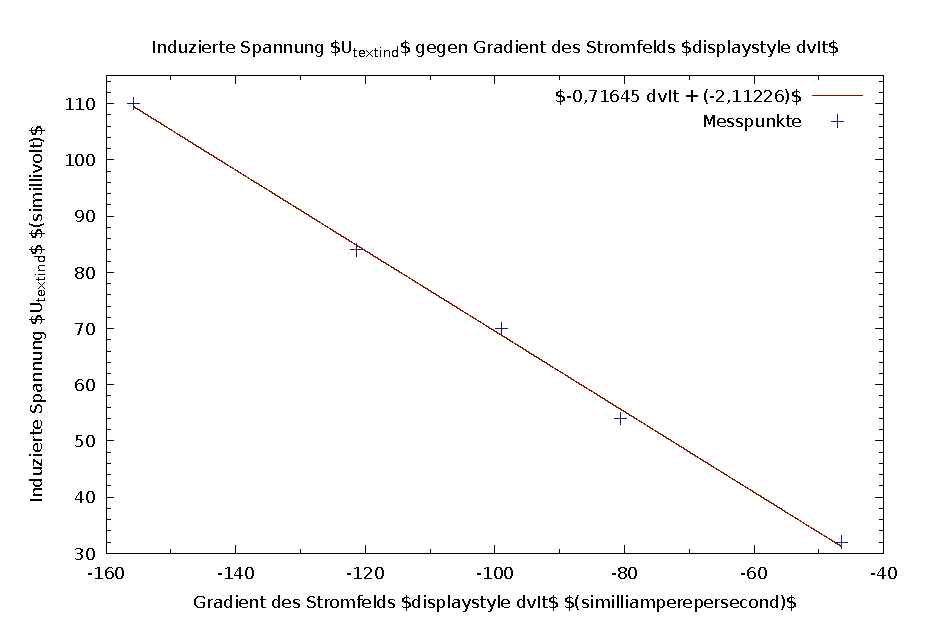
\includegraphics[width={432.00bp},height={288.00bp}]{tv4-plot}}%
    \gplfronttext
  \end{picture}%
\endgroup

		\caption{\centering Überprüfung des Induktionsgesetzes \captionbr $\chi^2_{\text{red}} = \num{1.89758} \implies$ Verträgliche Anpassung}
		\label{fig:tvfour-plot}
		\vspace{-1em}
	\end{figure}
	Als Endergebnis erhalten wir:
	\begin{equation*}
		\begin{tabu}{lll}
			\toprule
			\text{Variable} & \text{Wert} & \text{Gerundet} \\
			\midrule
			m & \SI{-0.71645(1671)}{\milli\volt\second\per\milli\ampere} & \SI{-0.716(17)}{\milli\volt\second\per\milli\ampere}\\
			c & \SI{-2.112(1791)}{\milli\volt} & \SI{-2.1(18)}{\milli\volt} \\
			\bottomrule
		\end{tabu}
	\end{equation*} 
	Die Gerade soll durch den Nullpunkt liegen, was verträglich mit unserem Ergebnis ist, da Null im Dreifachen des Fehlerintervalls von $c$ liegt. 

	Der theoretische Wert von $m$ ist gegeben durch:
	\begin{align}
		m &= -\left(\frac{4}{5}\right)^{\nicefrac{3}{2}} \frac{2\mu_0N_{\text{ind}}N\!A}{R} \\
		\Delta m &= m \frac{\Delta R}{R}
	\end{align}
	Mit der Werten:
	\begin{center}
		\begin{tabular}{lll}
			\toprule
			Variable & Wert & Bedeutung \\
			\midrule
			$R$ & \SI{27.57(5)}{\centi\meter} & Durchmesser der Helmholtzspule \\
			$A$ & \SI{23.5}{\centi\meter\squared} & Fläsche der Induktionsspule \\
			$N_\text{ind}$ & \SI{82800}{} & Windungszahl der Induktionsspule \\
			$N$ & \SI{528}{} & Windungszahl der Helmholtzspule \\
			$\mu_0$ & \SI{1.257e-6}{\newton\per\ampere\squared} & Magnetische Feldkonstante \\
			\bottomrule
		\end{tabular}
	\end{center}
	erhalten wir:
	\begin{align}
		m &= -\left(\frac{4}{5}\right)^{\nicefrac{3}{2}} \frac{2(\SI{1.257e-6}{\newton\per\ampere\squared})(\SI{82800}{})(\SI{528}{})(\SI{2.35e-3}{\meter\squared})}{(\SI{0.2757}{\meter})} \notag\\
		&= \SI{-0.670341}{\volt\second\per\ampere} \sigfig{6}\\
		\Delta m &= (\SI{0.670341}{\volt\second\per\ampere}) \frac{\SI{0.05}{\centi\meter}}{\SI{27.57}{\centi\meter}} = \SI{1.21571e-3}{\volt\second\per\ampere} \sigfig{6} \\
		\Rightarrow m &= \SI{-0.6703(13)}{\volt\second\per\ampere} = \SI{-0.6703(13)}{\milli\volt\second\per\milli\ampere}
	\end{align}